\documentclass[11pt]{article}
\usepackage{../EllioStyle}

\title{Homework 1}
\author{Elliott Pryor}
\date{28 Aug 2020}


\begin{document}
\maketitle

\problem{1.22}
Prove that the sum of the deviations of a set of measurements about their mean is equal to zero:
$$\sum_{i=1}^n (y_i - \bar{y}) = 0$$
\hrule

\begin{proof}
We show that the sum of the deviations of a set about the mean is equal to zero. We first give the definition of $\bar{y} = 1/n \sum_{i=1}^n y_i$. For conciseness, we also let $S = \sum_{i=1}^n y_i$

\begin{align*}
\sum_{i=1}^n (y_i - \bar{y}) &= 0\\
\sum_{i=1}^n y_i - \sum_{i=1}^n \bar{y} &= 0\\
S - \sum_{i=1}^n (1/n \sum_{i=1}^n y_i) &= 0\\
S - 1/n \sum_{i=1}^n S) &= 0\\
S - 1/n * n * S) &= 0\\
S - S &= 0\\
0 &= 0
\end{align*}

\end{proof}




\problem{2.23}
If A and B are events and $B \subset A$, why is it ``obvious" that $P(B) \leq P(A)$.
\hrule

Qualitatively if $B \subset A$ then everything in $B$ is also in $A$. So the probability that $A$ happens must be at least as big as $B$. 

Mathematically, we can also show this.
\begin{proof}
 We let $C = A \setminus B$. Then $A = B \cup C$, and $B \cap C = \emptyset$. So we can use the third axiom of probability to state that $P(A) = P(B) + P(C)$. Well $P(A) = P(B) + P(C) \geq P(B)$ as required.
\end{proof}
 
 
 
 
\problem{2.33}
The Bureau of the Census reports that the median family income for all families in the United
States during the year 2003 was \$43,318. That is, half of all American families had incomes
exceeding this amount, and half had incomes equal to or below this amount. Suppose that four
families are surveyed and that each one reveals whether its income exceeded \$43,318 in 2003
\begin{enumerate}[\textbf{a}]
 	\item List the points in the sample space
 	\item Identify the simple events in each of the following spaces.
 	
 	
		\quad $A$: \quad At least two had incomes exceeding \$43,318 	
 	
 		\quad $B$: \quad Exactly two had incomes exceeding \$43,318
 	
 		\quad $C$: \quad Exactly two had incomes less than or equal to \$43,318
 	
 	\item Make use of the given interpretation for the median to assign probabilities to simple events and find $P(A), P(B), P(C)$  
\end{enumerate}
\hrule

\begin{enumerate}[a]

	\item We say that $E$ represents if a family exceeded the median and $N$ if they did not exceed the median income. 
	
	\begin{multline*}
	\mathcal{S} = \{EEEE, EEEN, EENE, EENN, ENEE, ENEN, ENNE, ENNN, \\ 
	NEEE, NEEN, NENE, NENN, NNEE, NNEN, NNNE, NNNN\}
	\end{multline*}
	
	
	
	
	\item
	
	\quad \begin{multline*}
	A = \{EEEE, EEEN, EENE, EENN, ENEE, ENEN, ENNE, NEEE,\\
	 NEEN, NENE, NNEE\}
	\end{multline*}	
	
	\quad $B = \{EENN, ENEN, ENNE, NEEN, NENE, NNEE\}$
	
	\quad $C = \{EEEN, EENE, ENEE, NEEE\}$
	
	
	\item By definition of the median value, exactly half of the individuals will have incomes exceeding the median amount. So the probability that a family has $E$ is $0.5$. We assume that all families are equally likely to be above the median value. So all simple events have a probability of $0.5 * 0.5 *0.5 * 0.5 = 1/16$.
	
	$P(A) = 1/16 * |A| = 1/16 * 11 = 0.6875$ 
	
	$P(B) = 1/16 * |B| = 1/16 * 6 = 0.375$ 
	
	$P(C) = 1/16 * |C| = 1/16 * 4 = 0.25$ 

\end{enumerate}


\problem{6} Do R tutorial.
\hrule
No questions.

\problem{7}

Generate a random sample of size 24 from a normal distribution with mean = 21 and sd = 3, then add a 25th observation equal to 52.2

\begin{enumerate}[a.]

\item Construct a histogram
\item Calculate sample mean ($\bar{y}$) and standard deviation ($s$) for the whole sample ($n=25$)
\item Calculate the intervals $\bar{y} \pm ks$ for $k = 1,2,\text{ and } 3$.
\item Calculate the range of the set of values. Calculate an approximate value for $s$ using the calculated range and the empirical rule. Compare this to the $s$ you
calculated in (a).
\item Repeat part (a) after excluding the outlying observation. Are you surprised by how much the result changed?
\end{enumerate}
\hrule

\begin{enumerate}[a.]

\item 

\begin{figure}[h!]
    \centering
    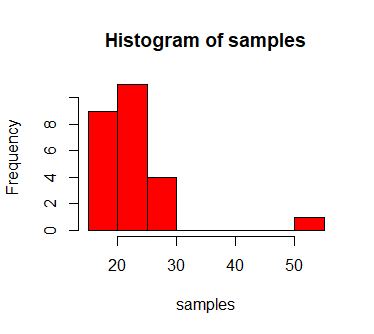
\includegraphics[scale=1]{./pics/histWithOutlier.png}
    \caption{Histogram of all 25 samples}
    \label{fig:histWith}
\end{figure}

\item $\bar{y} = 22.86172$, $s = 6.746023$

\item The intervals are $[16.115693, 29.60774], [9.369670, 36.35376], [2.623647, 43.09979]$ for $k = 1, 2, 3$ respectively.

\item The counts are 24 for every interval set, which is 96\%. This is more than expected from the empirical rule for the first two intervals which expects 68\%, 95\%, 99.7\% of the data in each interval. However, with only 25 sample points the measured percentage cannot go higher unless 100\% of the data points fall within a region.

\item  range $= 36.26181$. We then use the range rule $range = 4 * s$ to estimate $s$. We get $s = 9.065452$ using our estimate.

\item No I am not surprised. The outlier was very far removed from all of the other data points so significantly stretched the standard deviation. This makes the boxes bigger in the histogram so you cannot see the smaller variations within the 24 sample points.

\begin{figure}[h!]
    \centering
    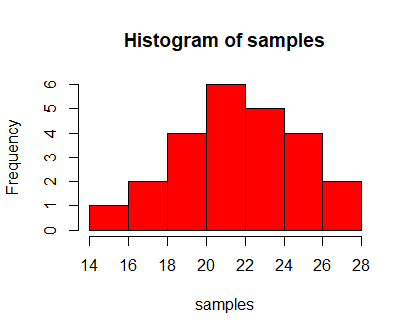
\includegraphics[scale=1]{./pics/histWithoutOutlier.png}
    \caption{Histogram with only 24 samples (no outlier)}
    \label{fig:histWithout}
\end{figure}

\end{enumerate}

\end{document}


